\documentclass[11pt]{article}
\usepackage[a4paper, left=0.75in, right=0.75in, top=0.5in, bottom=0.5in]{geometry}
\usepackage{amsmath, bm}
\usepackage{amssymb}
\usepackage{hyperref}
\usepackage{booktabs}
\hypersetup{
    colorlinks=true,
    linkcolor=blue,
    filecolor=magenta,      
    urlcolor=blue,
}
\usepackage{graphicx}
\graphicspath{ {.} }
\usepackage[backend=biber]{biblatex}
\addbibresource{my-paper.bib}


\title{MSE 402 - Assignment 3}
\date{}
\author{Nishant Tatar - 21110223}

\begin{document}
\maketitle

\section{Question 1}
As the cutoff energy is increased, the total ground state energy of the system decreases. However, the drop in the total ground state energy does not reflect the increasing cutoff energies, and starts converging to a value. This can be observed in the graph given below:\\
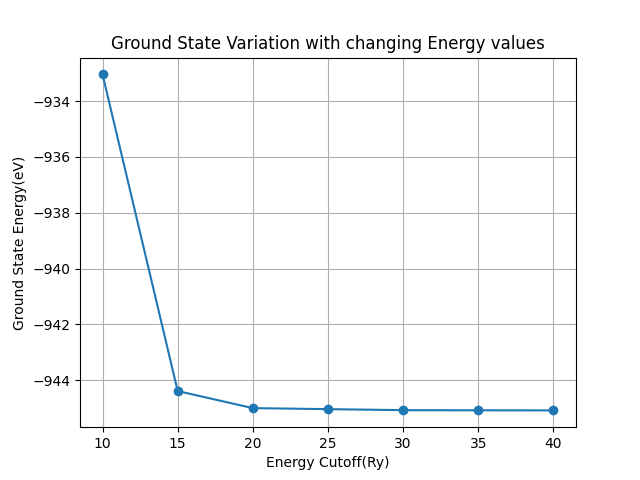
\includegraphics[scale=0.5]{Q1.png}\\
From the graph, we can take the cutoff energy to be 20Ry, to conserve computational power.

\section{Question 2}

\begin{table}[h!]
    \centering
    \begin{tabular}{l c c}
        \toprule
        \textbf{Mesh} & \textbf{Unique K Points} & \textbf{Energy (eV)} \\
        \midrule
        3 3 3 0 0 0  & 4.0   & -944.8523544844821 \\
        3 3 3 1 1 1  & 6.0   & -944.9838506201581 \\
        4 4 4 0 0 0  & 8.0   & -944.8180015785695 \\
        4 4 4 1 1 1  & 10.0  & -945.0006903999697 \\
        5 5 5 0 0 0  & 10.0  & -944.8971346658653 \\
        5 5 5 1 1 1  & 19.0  & -945.0000771908915 \\
        6 6 6 0 0 0  & 16.0  & -944.9761419003993 \\
        6 6 6 1 1 1  & 28.0  & -945.0041035268691 \\
        7 7 7 0 0 0  & 20.0  & -944.9743323417704 \\
        7 7 7 1 1 1  & 44.0  & -945.0040731861493 \\
        8 8 8 0 0 0  & 29.0  & -944.9911528014823 \\
        8 8 8 1 1 1  & 60.0  & -945.0044476151228 \\
        9 9 9 0 0 0  & 35.0  & -944.9954243122456 \\
        9 9 9 1 1 1  & 85.0  & -945.0043716952945 \\
        10 10 10 0 0 0 & 47.0 & -944.997923135838  \\
        10 10 10 1 1 1 & 110.0 & -945.0044161859464 \\
        \bottomrule
    \end{tabular}
    \caption{Energy Variation with Unique K Points for Different Directories}
    \label{table:energy_kpoints}
\end{table}

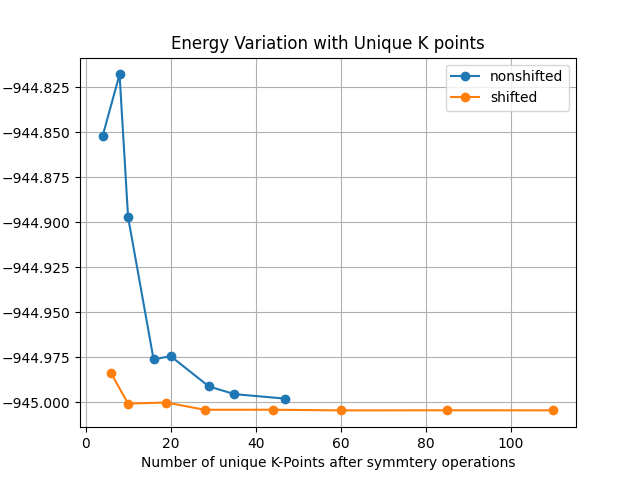
\includegraphics[scale=0.75]{Q2.png}\\
From here, we can see that irrespective of shifted or non shifted meshes, as the number of k points increases, the energy approaches a convergence. We can take the number of unique k points to be higher than 30, which compared to the table given, gives us 9 9 9 0 0 0 as one possible mesh size.

\section{Question 3}
Finding the Energies after varying the lattice parameters, we find the following energy graph:\\
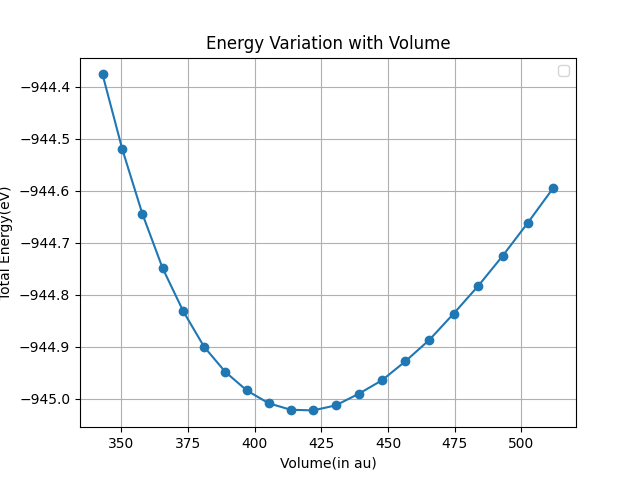
\includegraphics[scale=0.75]{Q3b.png}\\
The minima of the curve is the lattice paramter with the lowest equilibrium energy. Using $\textbf{ev.x}$, with fcc bravais lattice and using the birch equation of state, we find the minisation. This turns out to be \textbf{$7.4734355029$ Au}. The calculated value is higher than the experimental value which is given as $7.37 Au$.

\section{Question 4}

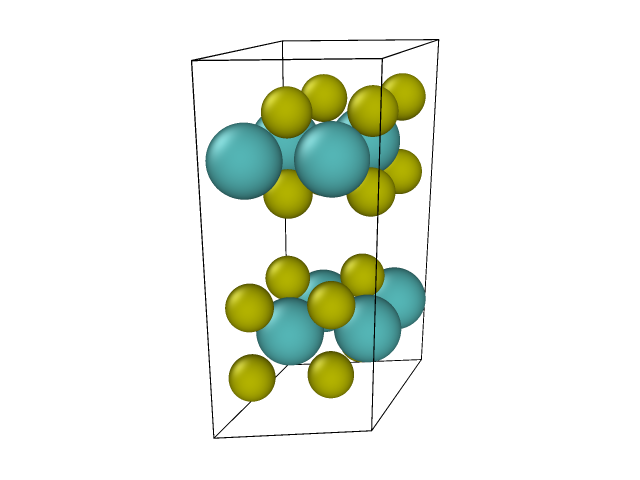
\includegraphics[scale=0.5]{MoS2.png}\\
MoS2 Visualised\cite{noauthor_undated-ej}

\subsection{A}
\begin{table}[h!]
    \centering
    \begin{tabular}{|c|c|c|}
    \hline
    \textbf{Iteration \#} & \textbf{Total Energy (Ry)} & \textbf{Estimated SCF Accuracy (Ry)} \\
    \hline
    1  & -57.59010641 & 8.57050880 \\
    2  & -54.77872243 & 90.24384911 \\
    3  & -63.16434532 & 2.12936424 \\
    4  & -63.34202784 & 0.44020926 \\
    5  & -63.41244093 & 0.06572166 \\
    13 & -63.43557995 & 0.00000220 \\
    14 & -63.43558023 & 0.00000005 \\
    15 & -63.43558028 & 0.00000002 \\
    16 & -63.43558028 & 9.6E-09 \\
    17 & -63.43558028 & 2.7E-09 \\
    \hline
    \end{tabular}
    \caption{Total Energy and Estimated SCF Accuracy per Iteration}
    \label{tab:scf_accuracy}
\end{table}

For the first few iterations, the calcuations try to converge towards a minimum value, where we can see the values deviate wildly, with a large accuracy value. However, as the values start to converge, as we can see in the last 5 iterations as the values of the estimated accuracy becomes lower and lower.

\subsection{B}
\begin{table}[h!]
    \centering
    \begin{tabular}{|l|r|r|}
    \hline
    \textbf{Type of Energy}       & \textbf{Energy (Ry)} & \textbf{Percentage of Total Energy (\%)} \\
    \hline
    Ewald contribution             & -47.83505156        & 75.39 \\
    Hartree contribution           &  26.32127989        & -41.49 \\
    One-electron contribution      & -23.98193456        & 37.81 \\
    XC contribution                & -17.93987405        & 28.29 \\
    \hline
    \textbf{Total Energy}          & -63.43558028        & 100.00 \\
    \hline
    \end{tabular}
    \caption{Energy Contributions and Their Percentage of the Total Energy}
    \label{tab:energy_contributions}
\end{table}

From the values we can see that all types of energy are important, and we cannot ignore any particular type of energy.

\subsection{C}
The band structure is found, given below:\\
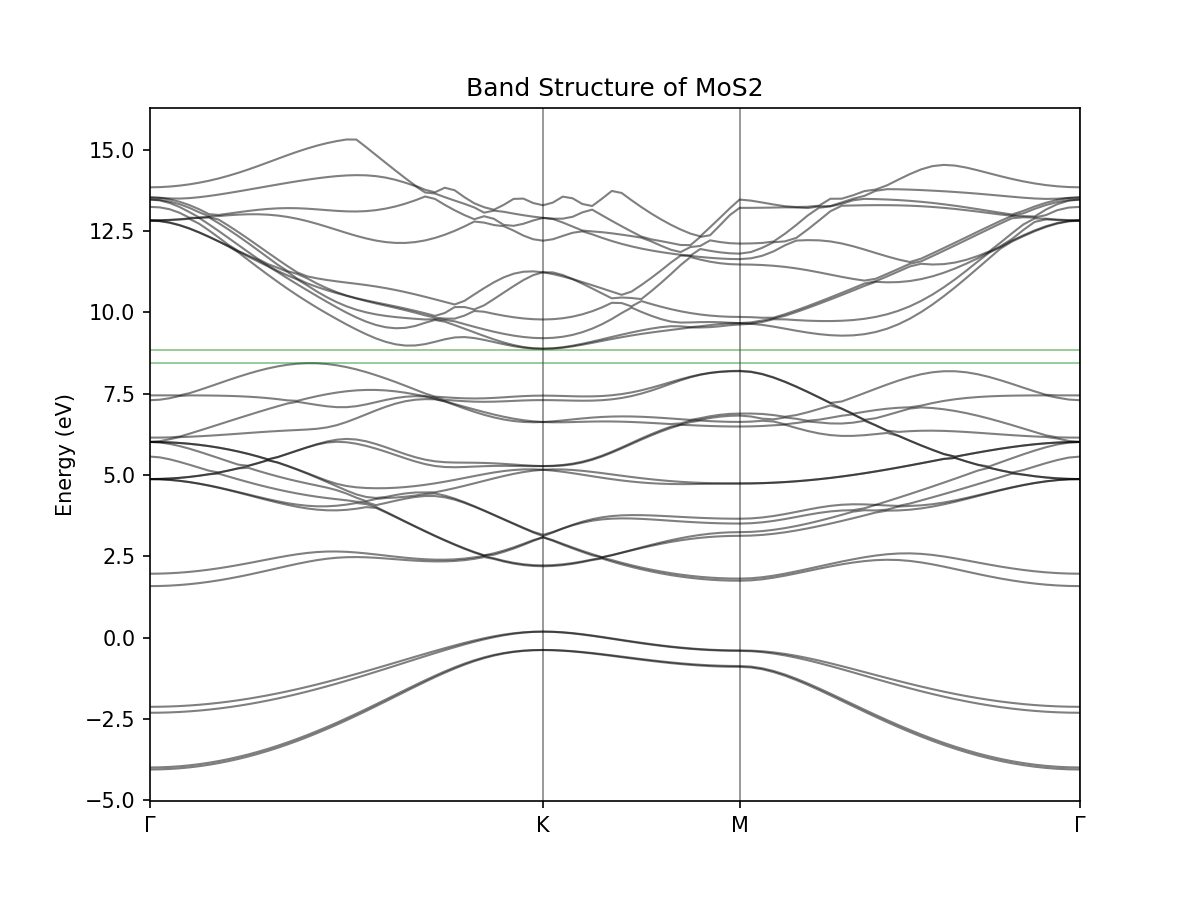
\includegraphics[scale=0.75]{Q4.png}\\
From here, as the band gap is the energy difference, the band gap difference comes around to be $\textbf{0.4}$ \text{eV}.

\printbibliography
\end{document}